% 2008 年湖北卷理科第 10 题：三条以 F 为焦点的轨道（椭圆 I、II 与圆 III）在 P 点相切。
% 来源 PDF：gaokaomath-src/普通高考/2008/2008湖北文.pdf
% SHA-256：54077e9ac5227f015a8972bfc4c4415b503b31acdf0a6e7cd51782afa098a112
% 原页：2008湖北理.pdf 第 1 页（A3 三栏）第 2 栏，书页码 449。
% 绘制依据：按原页 P 在最上方、F 在其下方，三条轨道在 P 处相切：椭圆 I 最大、II 次之，
%   圆 III 以 F 为圆心；贯穿 P、F 的对称轴用虚线，轨道编号标在右侧。
%   取 |PF|=1.5：椭圆 I 的 a=2.4、c=0.9；椭圆 II 的 a=1.9、c=0.4；圆 III 半径 1.5。
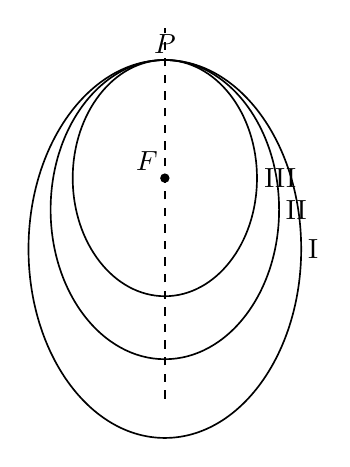
\begin{tikzpicture}[x=0.78cm, y=1.0cm, semithick, every node/.style={inner sep=1.3pt}]
  % 对称轴
  \draw[dashed] (0,-1.7) -- (0,3.0);

  % 椭圆 I：中心 (0,0.2)，半长轴 2.4、半短轴 2.22
  \draw (0,0.2) ellipse [x radius=2.22, y radius=2.4];
  % 椭圆 II：中心 (0,0.7)，半长轴 1.9、半短轴 1.86
  \draw (0,0.7) ellipse [x radius=1.86, y radius=1.9];
  % 圆 III：圆心 F(0,1.1)，半径 1.5
  \draw (0,1.1) circle [radius=1.5];

  % 焦点与切点
  \fill (0,1.1) circle (1.7pt);
  \node[above left=1pt] at (0,1.1) {$F$};
  \node[above] at (0,2.62) {$P$};

  \node[right] at (2.26,0.20) {I};
  \node[right] at (1.90,0.70) {II};
  \node[right] at (1.55,1.10) {III};
\end{tikzpicture}
